% !TeX spellcheck = es_ES
% !TEX encoding = UTF-8 Unicode
\documentclass[t, compress, spanish, aspectratio=169]{beamer}
%\documentclass[handout]{beamer}    % for the handout

\usetheme[progressbar=frametitle]{metropolis}

%\usetheme[secheader]{Madrid}
%\usetheme{Frankfurt}
%\usetheme{Warsaw}
%\usetheme{Berlin}
%\usetheme{CambridgeUS}

%\usecolortheme{beaver}     % Fondo Blanco y letras Negras - Titulos en Rojo con fondo gris
%\usecolortheme{dove}       % Para el Handout
%\usecolortheme{seahorse}   % Fondo Blanco y letras Negras - Titulos en Celeste
%\usecolortheme{dolphin}    % Fondo Blanco y letras Negras - Titulos en Celeste
%\usecolortheme{seagull}    % Fondo Blanco y letras Negras - Titulos en Gris
%\usecolortheme{crane}      % Fondo Blanco y letras Negras - Titulos en Amarillo
%\usecolortheme{wolverine}  % Fondo Blanco y Letras negras - Titulos en negro con fondo amarillo
%\usecolortheme{lily}       % Fondo Blanco y letras Negras - Titulos en Azul
%\usecolortheme{fly}        % Fondo Gris y letras Negras - Titulos en Rojo
%\usecolortheme{beetle}     % Fondo Gris y letras Negras - Titulos en blanco
%\usecolortheme{albatross}  % Fondo Azul y letras blancas
%\usecolortheme{orchid}     % Default
%\usecolortheme{rose}       % Default
%\usecolortheme{whale}      % Default

\setbeamertemplate{navigation symbols}{} % Gets rid of navigation symbols
%\setbeamercovered{transparent}

\usepackage{dsfont} % Double stroke fonts for math symbols
% \usepackage[T1]{fontenc}  % Helps with hyphenation for languages with accented characters. Note: Does not work with XeLaTex
% \usepackage[latin1]{inputenc} % Allows to type in latin (accents). Note: Does not work with XeLaTex
% \usefonttheme[onlymath]{serif}  % Changes fonts for math to serif
\usepackage[english]{babel} % Manages differences between languages: hyphenation etc

\usepackage{appendixnumberbeamer} % Does not include backup slides in the number of pages

\usepackage{centernot} % To draw not in math symbols (does not imply)

\usepackage{ragged2e}  % Text alignment
\justifying

\usepackage{graphicx} % Format for graphics: additional options for includefigure
\usepackage{pgf} % Tool for graphics

\usepackage{booktabs} % Format for tables: top, bottom and mid lines
\usepackage[scale=2]{ccicons}
\usepackage{threeparttable} % Format for tables
\usepackage{lscape} % Landscape for tables

% Customized commands
  \newcommand{\vs}{\vskip0pt plus.5fill}
  \newcommand{\SR}{\mathbb{R}}
  \DeclareMathOperator{\plim}{plim}
  \DeclareMathOperator{\Var}{Var}
  \DeclareMathOperator{\Avar}{AVar}
  \DeclareMathOperator{\Cov}{Cov}
  \DeclareMathOperator{\N}{Normal}
  \DeclareMathOperator{\E}{\mathbb{E}}
  \DeclareMathOperator{\LP}{\mathbb{L}}
  \newcommand{\pto}{\stackrel{p}{\longrightarrow}}
  \newcommand{\dto}{\stackrel{d}{\longrightarrow}}
  \newcommand{\adistr}{\stackrel{a}{\sim}}
  \newcommand{\epsi}{\varepsilon}
  \newcommand{\tmle}{\hat \theta_{ML}}
  \newcommand{\tgmm}{\hat \theta_{GMM}}
  \newcommand\independent{\protect\mathpalette{\protect\independenT}{\perp}}
  \def\independenT#1#2{\mathrel{\rlap{$#1#2$}\mkern2mu{#1#2}}}

\title [Inferencia MCO] {Econometr\'ia I\\
 Modelo Lineal de Regresi\'on: Inferencia por MCO}
\author[de Elejalde]{Ramiro de Elejalde}
\institute [UAH] {Facultad de Econom\'ia y Finanzas \\ Universidad Alberto Hurtado}
\date[\today] {}
\subject{Econometr\'ia}
\begin{document}
	
%------------------------------------------------------------

\begin{frame}
    \titlepage
\end{frame}

% --------------------------------------------------- Slide --
\begin{frame}
	\frametitle{Outline}
	\tableofcontents
	\alert{Referencias}: Cap. 7 y 9 de Hansen, cap. 3.5.2 y 4.2.3 de Wooldridge, y cap. 7 de Stock and Watson.
\end{frame}
%% --------------------------------------------------- Slide --
%\section[Motivaci\'on: Tama\~no de clase y rendimiento acad\'emico]{Motivaci\'on: Efecto del tama\~no de clase en el rendimiento aca--d\'emico (California)}
%\begin{frame}
%    \frametitle{Efecto del tama\~no de clase en el rendimiento acad\'emico (California)}
%    \begin{itemize}
%        \item \alert{Pregunta de pol\'itica}: ?`Cu\'al es el efecto de reducir el tama\~no de clase en el rendimiento escolar?
%        \item \alert{Datos}: Todos los distritos escolares de escuelas K-6 y K-8 de California ($N=420$)
%        \item \alert{Variables}:
%        \begin{itemize}
%            \item Notas de examen de 5to grado (Stanford-9 achievement test, matem\'atica y lectura), media del distrito (\emph{testscr})
%            \item Ratio estudiantes/maestros: n\'umero de estudiantes en el distrito divido por el n\'umero de maestros tiempo completo (\emph{str}).
%        \end{itemize}
%    \end{itemize}
%\end{frame}
%% --------------------------------------------------- Slide --
%\begin{frame}
%\frametitle{Modelo poblacional}
%    \begin{itemize}
%        \item []
%        \begin{align*}
%            testscr_i = \beta_0 + \beta_1 \, str_i+\beta_2 \,el\_pct_i+u_i,
%        \end{align*}
%        donde $u_i$ contiene todos los factores que influyen sobre el rendimiento escolar adem\'as de las variables explicativas incluidas en el modelo.
%    \end{itemize}
%\end{frame}
%% --------------------------------------------------- Slide --
%\begin{frame}
%\frametitle{Modelo poblacional}
%    \begin{itemize}
%        \item []
%        \begin{align*}
%            testscr_i = \beta_0 + \beta_1 \, str_i+\beta_2 \,el\_pct_i+u_i
%        \end{align*}
%        \item Supuestos:
%        \begin{enumerate}
%            \item [OLS1] Muestra aleatoria
%            \item [OLS2] No correlaci\'on entre variables explicativas y error: $\E(x_iu_i)=0$.
%            \item [OLS3] No multicolinealidad perfecta entre las variables explicativas.
%            \item [OLS4] ``No fat tails'': los valores at\'ipicos son poco probables.
%        \end{enumerate}
%        \item \alert{Intuici\'on}: Controlar por variables observables para hacer estudiantes en distintos tama\~nos de clase comparables. Buscamos generar \alert{asignaci\'on aleatoria condicional en observables.}
%    \end{itemize}
%\end{frame}
%% --------------------------------------------------- Slide --
%\begin{frame}
%    \frametitle{Estimaci\'on por MCO}
%    \begin{itemize}
%        \bigskip
%        \item \alert{Consistencia}: $\plim \hat \beta = \beta$.
%        \item \alert{Distribuci\'on asint\'otica normal}: $\sqrt{N}(\hat \beta - \beta)\dto \N(0,V)$ donde $V=\Avar(\sqrt{N}(\hat \beta - \beta))$.
%        \item \alert{Estimaci\'on consistente de la matriz de varianzas-covarianzas}: $\plim \hat V = V$.
%        \item Usando estos resultados,
%        \begin{align*}
%            	&\hat \beta \adistr \N(\beta,\frac{V}{N}), \text{y}\\
%            	&s.e.(\hat \beta_j ) = \frac{\hat v_{jj}^{1/2}}{N^{1/2}} \quad \text{donde } v_{jj} \text{ es el elemento } jj \text{ de }V.
%        \end{align*}
%    \end{itemize}
%\end{frame}

% --------------------------------------------------- Slide --
\begin{frame}[fragile]
\frametitle{Estimaci\'on MCO: Tama\~no de clase y rendimiento acad\'emico}
Salida de Stata
\tiny{
\begin{verbatim}
    .     reg testscr str  el_pct, robust
    
    Linear regression                                      Number of obs =     420
                                                           F(  2,   417) =  223.82
                                                           Prob > F      =  0.0000
                                                           R-squared     =  0.4264
                                                           Root MSE      =  14.464
    
    ------------------------------------------------------------------------------
                 |               Robust
         testscr |      Coef.   Std. Err.      t    P>|t|     [95% Conf. Interval]
    -------------+----------------------------------------------------------------
             str |  -1.101296   .4328472    -2.54   0.011     -1.95213   -.2504616
          el_pct |  -.6497768   .0310318   -20.94   0.000     -.710775   -.5887786
           _cons |   686.0322   8.728224    78.60   0.000     668.8754     703.189
    ------------------------------------------------------------------------------
\end{verbatim}
}
\end{frame}
% --------------------------------------------------- Slide --
\begin{frame}
\frametitle{Contraste de hip\'otesis e intervalos de confianza}
    \begin{itemize}
        \item En esta unidad vamos a estudiar como incorporar la influencia de la aleatoriedad muestral en el an\'alisis de los resultados.
        \bigskip
        \begin{enumerate}
            \item [] $\implies$ \alert{Contraste de hip\'otesis}
            \bigskip
            \item [] $\implies$ \alert{Intervalos de confianza}
        \end{enumerate}
    \end{itemize}
\end{frame}
% --------------------------------------------------- Slide --
\section{Contraste de una restricci\'on lineal sobre un par\'ametro}
% --------------------------------------------------- Slide --
\begin{frame}
\frametitle{Contraste de una restricci\'on lineal sobre un par\'ametro}
        \begin{itemize}
            \item [] \alert{Hip\'otesis nula}
            \begin{align*}
                H_0: \beta_j = \beta_{j,0}.
            \end{align*}
            \item [] \alert{Hip\'otesis alternativa}
            \begin{align*}
                H_1: \beta_j \neq \beta_{j,0}.
            \end{align*}
        \end{itemize}
\end{frame}
% --------------------------------------------------- Slide --
\begin{frame}
%\frametitle{Contraste de una restricci\'on lineal sobre un par\'ametro}
        \begin{itemize} 
            \item <1-> \alert{Regla de decisi\'on}: Un estad\'istico $T_N$, un valor cr\'itico $c_\alpha$ y una regla de decisi\'on:
            \begin{enumerate}
                \item No rechazar $H_0$ si $T_N \leq c_\alpha$,
                \item Rechazar $H_0$ si $T_N >c_\alpha$.
            \end{enumerate}
            \item <2-> \alert{Test estad\'istico}: Estad\'istico t en valor absoluto
            \begin{align*}
                |t_N|=\left|\frac{\hat \beta_j-\beta_{j,0}}{s.e.(\hat \beta_j)}  \right|
              \end{align*}
        \end{itemize}
\end{frame}

%\begin{frame}
%\frametitle{Contraste de hip\'otesis}
%        \begin{itemize}
%            \item Dados unos par\'ametros $\theta \in \Theta$.
%            \item  [] \alert{Hip\'otesis nula}
%            \begin{align*}
%                H_0: \theta = \theta_0.
%            \end{align*}
%            \item  [] \alert{Hip\'otesis alternativa}
%            \begin{align*}
%                H_1: \theta \neq \theta_0,
%            \end{align*}
%            \item  Regla de decisi\'on: Un \alert{estad\'istico} $T_N$, un \alert{valor cr\'itico} $c_\alpha$ y una \alert{regla de decisi\'on}:
%            \begin{enumerate}
%                \item No rechazar $H_0$ si $T_N \leq c_\alpha$,
%                \item Rechazar $H_0$ si $T_N >c_\alpha$.
%            \end{enumerate}        
%        \end{itemize}
%            % Ejemplo: Test \beta_1=0 vs una cola y dos colas 
%            % Queremos buscar evidencia en la muestra que respalde la hip\'otesis nula o la hip\'otesis alternativa.
%            % Ejemplo: Test \beta_1=0 vs una cola y dos colas 
%            % Estadistico t: Para dos colas |t_N|, para una cola t_N \'o -t_N.
%\end{frame}
% --------------------------------------------------- Slide --
\begin{frame}
	\frametitle{Error tipo I y tama\~no del test}
	\begin{table}
		\scriptsize
		\begin{tabular} {l c c}
			\toprule
			&   \multicolumn{2}{c}{Decisi\'on en el contraste de hip\'otesis}   \\
			\cmidrule(r){2-3}
			& No rechazar $H_0$     & Rechazar $H_0$		\\
			\midrule
			$H_0$ es verdadera	& Decisi\'on correcta &      \alert{Error tipo I	}	\\
			$H_1$ es verdadera  & Error tipo II     & Decisi\'on correcta 	\\
			\bottomrule
		\end{tabular}
	\end{table}
	\small
	% Al fijar el error tipo I, fijamos el valor cr\'itico $c_\alpha$.
	\begin{itemize}
		\item <1-> El \alert{tama\~no del test} es la probabilidad del error tipo I. El  \alert{tama\~no asint\'otico del test} $\alpha$ es dicha probabilidad en el l\'imite:
	\begin{align*}
    \lim_{N\to \infty}\Pr(\text{Rechazar }H_0|H_0 )=&\lim_{N\to \infty}\Pr(T_N >c_\alpha|H_0)
    =\Pr(T >c_\alpha) = \alpha\\
    &\text{ donde } T_N\dto T \text{ bajo } H_0.
    \end{align*}
	\end{itemize}
\end{frame}
% --------------------------------------------------- Slide --
\begin{frame}
	\frametitle{Error tipo I y tama\~no del test}
	\begin{table}
		\scriptsize
		\begin{tabular} {l c c}
			\toprule
			&   \multicolumn{2}{c}{Decisi\'on en el contraste de hip\'otesis}   \\
			\cmidrule(r){2-3}
			& No rechazar $H_0$     & Rechazar $H_0$		\\
			\midrule
			$H_0$ es verdadera	& Decisi\'on correcta &      \alert{Error tipo I	}	\\
			$H_1$ es verdadera  & Error tipo II     & Decisi\'on correcta 	\\
			\bottomrule
		\end{tabular}
	\end{table}
	\small
	% Al fijar el error tipo I, fijamos el valor cr\'itico $c_\alpha$.
	\begin{itemize}
		\item Clave: Buscar $T_N$ cuya distribuci\'on asint\'otica bajo $H_0$ sea conocida.
		\item Si la distribuci\'on asint\'otica de $T_N$ no depende de par\'ametros desconocidos, el estad\'istico es \alert{asint\'oticamente pivotal}.
		\item Fijamos $\alpha$ y obtenemos $c_\alpha$ de la distribuci\'on asint\'otica de $T_N$.
	\end{itemize}
\end{frame}
% --------------------------------------------------- Slide --
\begin{frame}
%\frametitle{Una restricci\'on lineal sobre un par\'ametro}
        \begin{itemize}
            \item <1-> \alert{Test estad\'istico}: Estad\'istico t en valor absoluto
            \begin{align*}
                |t_N|=\left|\frac{\hat \beta_j-\beta_{j,0}}{s.e.(\hat \beta_j)} \right| \dto_{H_0} |Z|,
            \end{align*}
             donde $Z \sim \N(0,1)$ y $\Pr(|Z|\leq u)=2\Phi(u)-1$
        \end{itemize}
\end{frame}
%
%\begin{frame}
%\end{frame}
%
%\begin{frame}
%\end{frame}
%
%\begin{frame}
%\end{frame}
%
%
%\begin{frame}
%\end{frame}

\begin{frame}
%\frametitle{Una restricci\'on lineal sobre un par\'ametro}
        \begin{itemize}
            \item \alert{Test estad\'istico}: Estad\'istico t en valor absoluto
            \begin{align*}
                |t_N|=\left|\frac{\hat \beta_j-\beta_{j,0}}{s.e.(\hat \beta_j)} \right| \dto_{H_0} |Z|,
            \end{align*}
             donde $Z \sim \N(0,1)$ y $\Pr(|Z|\leq u)=2\Phi(u)-1$
            \item []  \alert{Demostraci\'on}:
            \begin{align*}
                t_N&=\frac{\hat \beta_j-\beta_{j,0}}{s.e.(\hat \beta_j)},\\
                   &=\sqrt{N}\frac{\hat \beta_j-\beta_{j,0}}{\hat v_{jj}^{1/2}},\\
                   &=\sqrt{N}\frac{\hat \beta_j-\beta_{j,0}}{v_{jj}^{1/2}}\frac{v_{jj}^{1/2}}{\hat v_{jj}^{1/2}}\dto_{H_0} Z \sim \N(0,1),
            \end{align*}
            usando el teorema de Slutsky y la distribuci\'on  asint\'otica normal.
        \end{itemize}
\end{frame}

% --------------------------------------------------- Slide --
\begin{frame}
%	\frametitle{Una restricci\'on lineal sobre un par\'ametro}
	\begin{itemize}
		\item  \alert{Test estad\'istico}: Estad\'istico t en valor absoluto
		\begin{align*}
		|t_N|=\left|\frac{\hat \beta_j-\beta_{j,0}}{s.e.(\hat \beta_j)} \right| \dto_{H_0} |Z|
		\end{align*}
         donde $Z \sim \N(0,1)$ y $\Pr(|Z|\leq u)=2\Phi(u)-1$.
		\item []  \alert{Demostraci\'on}:
		\begin{align*}
		t_N\dto_{H_0} Z \sim \N(0,1),
		\end{align*}
		entonces utilizando el TFC
		\begin{align*}
		|t_N|\dto_{H_0} |Z| \quad \text{donde } Z \sim \N(0,1).
		\end{align*}
		La probabilidad acumulada de $|Z|$ viene dada por
		\begin{align*}
		\Pr(|Z|\leq u)&=\Pr(-u\leq Z \leq u)\\
		 &= \Phi(u)-\Phi(-u) =\Phi(u)-(1-\Phi(u))\\
		 &=2\Phi(u)-1.
		\end{align*}
	\end{itemize}
\end{frame}
% --------------------------------------------------- Slide --
\begin{frame}
%\frametitle{Una restricci\'on lineal sobre un par\'ametro}
\small
        \begin{itemize}
            \item \alert{Test estad\'istico}: Estad\'istico t en valor absoluto
            \begin{align*}
            |t_N|=\left|\frac{\hat \beta_j-\beta_{j,0}}{s.e.(\hat \beta_j)} \right| \dto_{H_0} |Z|,
            \end{align*}
            donde $Z \sim \N(0,1)$ y $\Pr(|Z|\leq u)=2\Phi(u)-1$.
            \item  \alert{Valor cr\'itico} $c_\alpha=z_{1-\alpha/2}$ donde  $\alpha$ es el tama\~no del test y $\Phi(z_{1-\alpha/2})=1-\alpha/2$.
            \item [] <2->  \alert{Demostraci\'on}:
            \begin{align*}
                \lim_{N\to \infty}\Pr(\text{Rechazar }H_0|H_0)=\lim_{N\to \infty}\Pr(|t_N| >c_\alpha|H_0)= \Pr(|Z| >c_\alpha)=\alpha.
            \end{align*}
            Pero 
            \begin{align*}
            \Pr(|Z| >c_\alpha)&=1-\Pr(|Z| \leq c_\alpha)\\
            &=1-(2\Phi(c_\alpha)-1)=2(1-\Phi(c_\alpha))=\alpha\\
            &\iff \Phi(c_\alpha)=1-\alpha/2\\
            &\iff c_\alpha=z_{1-\alpha/2}
            \end{align*}
        \end{itemize}
\end{frame}
% --------------------------------------------------- Slide --
\begin{frame}
%	\frametitle{Una restricci\'on lineal sobre un par\'ametro}
	\begin{itemize}
		\item \alert{Test estad\'istico}: Estad\'istico t en valor absoluto
		\begin{align*}
		|t_N|=\left|\frac{\hat \beta_j-\beta_{j,0}}{s.e.(\hat \beta_j)} \right| \dto_{H_0} |Z|,
		\end{align*}
		donde $Z \sim \N(0,1)$ y $\Pr(|Z|\leq u)=2\Phi(u)-1$.
		\item  \alert{Valor cr\'itico} $c_\alpha=z_{1-\alpha/2}$ donde  $\alpha$ es el tama\~no del test.
		
		Si $\alpha=0.05$, entonces $c_\alpha=z_{0.975}=1.96$.
		\item \alert{Regla de decisi\'on}: Si $|t_N|>z_{1-\alpha/2}$, rechazamos $H_0$.
		
		Cuando rechazamos la hip\'otesis nula $H_0:  \beta_j=0$, solemos decir que $\beta_j$ es \alert{estad\'isticamente significativo}.
	\end{itemize}
\end{frame}

% --------------------------------------------------- Slide --
\begin{frame}
\frametitle{Ejemplo: Tama\~no de clase y rendimiento acad\'emico}
        \begin{itemize}
            \item Modelo
            \begin{align*}
                testscr_i = \beta_0 + \beta_1 \, str_i+\beta_2 el\_pct_i+u_i,
            \end{align*}
            \item \alert{Hip\'otesis nula}: El tama\~no de clase no tiene  efecto sobre el rendimiento acad\'emico.\\
            Formalmente:
            \begin{align*}
                H_0: \beta_1=0.
            \end{align*}
            \item \alert{Hip\'otesis alternativa}: El tama\~no de clase tiene efecto sobre el rendimiento acad\'emico.\\
            Formalmente:
            \begin{align*}
                H_1: \beta_1 \neq 0.
            \end{align*}
        \end{itemize}
\end{frame}
% --------------------------------------------------- Slide --
\begin{frame}[fragile]
\frametitle{Tama\~no de clase y rendimiento acad\'emico}
Salida de Stata\\
\tiny{
\begin{verbatim}
    .     reg testscr str  el_pct, robust
    
    Linear regression                                      Number of obs =     420
                                                           F(  2,   417) =  223.82
                                                           Prob > F      =  0.0000
                                                           R-squared     =  0.4264
                                                           Root MSE      =  14.464
    
    ------------------------------------------------------------------------------
                 |               Robust
         testscr |      Coef.   Std. Err.      t    P>|t|     [95% Conf. Interval]
    -------------+----------------------------------------------------------------
             str |  -1.101296   .4328472    -2.54   0.011     -1.95213   -.2504616
          el_pct |  -.6497768   .0310318   -20.94   0.000     -.710775   -.5887786
           _cons |   686.0322   8.728224    78.60   0.000     668.8754     703.189
    ------------------------------------------------------------------------------
\end{verbatim}
}
\normalsize
\begin{itemize}
    \item Significancia estad\'istica y significancia econ\'omica.
\end{itemize}
\end{frame}

% --------------------------------------------------- Slide --
\begin{frame}
\frametitle{p-valor}
    El \alert{p-valor} se define como $p_N=\Pr(T> T_N)$ donde $T_N\dto_{H_0} T$.
        \begin{itemize} [<+->]
            \item \alert{Intuici\'on}: La regla de decisi\'on es rechazar $H_0$ si $T_N>c_\alpha$ donde $\Pr(T>c_\alpha)=\alpha$. Una regla de decisi\'on equivalente es calcular el p-valor $\Pr(T>T_N)=p_N$ y rechazar si $p_N<\alpha$.
        \end{itemize}
\end{frame}

%\begin{frame}
%\frametitle{p-valor}
%\end{frame}
%
%\begin{frame}
%\frametitle{p-valor}
%\end{frame}


\begin{frame}
\frametitle{p-valor}
    El \alert{p-valor} se define como $p_N=\Pr(T> T_N)$ donde $T_N\dto_{H_0} T$.
        \begin{itemize} 
            \item \alert{Intuici\'on}: La regla de decisi\'on es rechazar $H_0$ si $T_N>c_\alpha$ donde $\Pr(T>c_\alpha)=\alpha$. Una regla de decisi\'on equivalente es calcular el p-valor $\Pr(T>T_N)=p_N$ y rechazar si $p_N<\alpha$.
            \item Dado que $\Pr(T>T_N)$ es decreciente en $T_N$, el p-valor  es una transformaci\'on mon\'otona de $T_N$ y por lo tanto es un estad\'istico equivalente. 
            \item \alert{El p-valor es el nivel de significatividad marginal}: el mayor valor de $\alpha$ tal que se rechaza $H_0$.
            \item  Para $H_0: \beta_j = \beta_{j,0}$ y $H_1: \beta_j \neq \beta_{j,0}$ con el estad\'istico t tenemos:
            \begin{align*}
                p_N&=\Pr(T> T_N)=\Pr(|Z|>|t_N|)=2(1-\Phi(|t_N|)).
            \end{align*}
        \end{itemize}
\end{frame}
% --------------------------------------------------- Slide --
\begin{frame}[fragile]
\frametitle{Tama\~no de clase y rendimiento acad\'emico}
Salida de Stata\\
\tiny{
\begin{verbatim}
    .     reg testscr str  el_pct, robust
    
    Linear regression                                      Number of obs =     420
                                                           F(  2,   417) =  223.82
                                                           Prob > F      =  0.0000
                                                           R-squared     =  0.4264
                                                           Root MSE      =  14.464
    
    ------------------------------------------------------------------------------
                 |               Robust
         testscr |      Coef.   Std. Err.      t    P>|t|     [95% Conf. Interval]
    -------------+----------------------------------------------------------------
             str |  -1.101296   .4328472    -2.54   0.011     -1.95213   -.2504616
          el_pct |  -.6497768   .0310318   -20.94   0.000     -.710775   -.5887786
           _cons |   686.0322   8.728224    78.60   0.000     668.8754     703.189
    ------------------------------------------------------------------------------
\end{verbatim}
}
\end{frame}
% --------------------------------------------------- Slide --

\begin{frame}
	\frametitle{Error tipo II y poder del test}
	\begin{table}
		\scriptsize
		\begin{tabular} {l c c}
			\toprule
			&   \multicolumn{2}{c}{Decisi\'on en el contraste de hip\'otesis}   \\
			\cmidrule(r){2-3}
			& No rechazar $H_0$     & Rechazar $H_0$		\\
			\midrule
			$H_0$ es verdadera	& Decisi\'on correcta &      Error tipo I		\\
			$H_1$ es verdadera  & \alert{Error tipo II}     & Decisi\'on correcta 	\\
			\bottomrule
		\end{tabular}
	\end{table}
	\small
	% Al fijar el error tipo I, fijamos el valor cr\'itico $c_\alpha$.
	\begin{itemize}
		\item El \alert{poder del test} $\pi_N(\beta_j)$ es uno menos la probabilidad del error tipo II:
		\begin{align*}
    			\Pr(\text{Rechazar }H_0|H_1)&=\Pr(T_N >c_\alpha|H_1)=\pi_N(\beta_j).
    		\end{align*}
		\item <2- > En general, el poder del test aumenta a medida que $\beta_j$ se aleja de $\beta_{j,0}$ y a medida que el tama\~no de la muestra aumenta.
		\item <2- > El objetivo en la construcci\'on del test es obtener un poder alto sujeto al tama\~no del test.
		\item <2- > Si el poder es igual al tama\~no del test, el test no provee informaci\'on sobre la hip\'otesis de inter\'es.
	\end{itemize}
\end{frame}

%\begin{frame}
%	\frametitle{Error tipo II y poder del test}
%\end{frame}
%
%\begin{frame}
%	\frametitle{Error tipo II y poder del test}
%\end{frame}

\begin{frame}
	\frametitle{Consistencia}
	\begin{itemize}
		\item  \alert{Consistencia} frente a la alternativa fija $H_1$: Si rechazamos con probabilidad uno bajo $H_1$ cuando $N \to \infty$,
		\begin{align*}
		\lim_{N\to \infty}\pi_N(\beta_j) &= \lim_{N\to \infty}\Pr(\text{Rechazar }H_0|H_1 ) \\
		&=\lim_{N\to \infty}\Pr(T_N >c_\alpha|H_1) \\
		& =1.
		\end{align*}
	\end{itemize}
	% Es parecido al poder del test
	% Algo m\'as parecido al poder, es comparar su comportamiento frente a alternativas que convergen a la nula a la misma velocidad que el test N^{1/2}: Pitman alternatives.
\end{frame}

\begin{frame}
\frametitle{Consistencia}
        \begin{itemize}
		\item \alert{Test estad\'istico}: Estad\'istico t en valor absoluto
		\begin{align*}
		|t_N|=\left|\frac{\hat \beta_j-\beta_{j,0}}{s.e.(\hat \beta_j)} \right| \dto_{H_0} |Z|,
		\end{align*}
		donde $Z \sim \N(0,1)$ y $\Pr(|Z|\leq u)=2\Phi(u)-1$.
            \item El contraste con el test estad\'istico t es \alert{consistente}.
        \end{itemize}
\end{frame}

%\begin{frame}
%\end{frame}

\begin{frame}
\frametitle{Consistencia}
        \begin{itemize}
		\item \alert{Test estad\'istico}: Estad\'istico t en valor absoluto
		\begin{align*}
		|t_N|=\left|\frac{\hat \beta_j-\beta_{j,0}}{s.e.(\hat \beta_j)} \right| \dto_{H_0} |Z|,
		\end{align*}
		donde $Z \sim \N(0,1)$ y $\Pr(|Z|\leq u)=2\Phi(u)-1$.
            \item El contraste con el test estad\'istico t es \alert{consistente}.
            \item [] \alert{Demostraci\'on}
            \begin{align*}
                t_N&=\frac{\hat \beta_j-\beta_{j,0}}{s.e.(\hat \beta_j)}=\frac{\hat \beta_j-\beta_{j}}{s.e.(\hat \beta_j)}+\sqrt{N}\frac{\beta_j-\beta_{j,0}}{\hat v_{jj}^{1/2}}\\
                &\dto_{H_1} \left\{
                \begin{array}{l c}
                    Z + \infty & \text{si }  \beta_j>\beta_{j,0},\\
                    Z -\infty & \text{si }  \beta_j<\beta_{j,0}.
                \end{array}
                \right.
                \text{ donde }Z\sim \N(0,1).
            \end{align*}
            $\lim_{N\to \infty}\Pr(|t_N| > z_{1-\alpha/2}|H_1)=\Pr(|Z\pm\infty| > z_{1-\alpha/2}|H_1)=1$
        \end{itemize}
\end{frame}

\begin{frame}
	\frametitle{Poder asint\'otico local}
	\begin{itemize} 
		\item Consistencia es un requisito m\'inimo para una test, pero no es una buena aproximaci\'on al poder del test.
		\item Una \alert{alternativa local} es una hip\'otesis alternativa $H_{1,N}$ que converge a $H_0$ a cierta velocidad. En este caso, $\beta_{j,N}=\beta_{j,0}+N^{-1/2}h$ donde $h$ es un par\'ametro.
		\item El \alert{poder asint\'otico local} de un test es el l\'imite cuando $N\to \infty$ del poder del test bajo la alternativa local:
		\begin{align*}
		\lim_{N\to \infty}\Pr(\text{Rechazar }H_0|H_{1,N})=\lim_{N\to \infty}\Pr(T_N >c_\alpha|H_{1,N}).
		\end{align*}
	\end{itemize}
	% Es parecido al poder del test
	% Algo m\'as parecido al poder, es comparar su comportamiento frente a alternativas que convergen a la nula a la misma velocidad que el test N^{1/2}: Pitman alternatives.
\end{frame}

\begin{frame}
%	\frametitle{Poder asint\'otico local}
	\begin{itemize}
		\item \alert{Poder asint\'otico local del test es decreciente en $v_{jj}$}
        \item [] Dada la alternativa local $H_{1,N}: \beta_{j,N}=\beta_{j,0}+N^{-1/2}h$, el poder asint\'otico es 
        $\lim_{N\to \infty}\Pr(|t_N| > z_{1-\alpha/2}|H_{1,N})=\Phi(\delta-c_\alpha)+\Phi(-\delta-c_\alpha)$ donde $\delta=h/v_{jj}^{1/2}$. El poder local es decreciente en $v_{jj}$(dado h) .
	\end{itemize}
\end{frame}
%
%\begin{frame}
%\end{frame}
%
%\begin{frame}
%\end{frame}

\begin{frame}
%	\frametitle{Poder asint\'otico local}
	\begin{itemize}
		\item \alert{Poder asint\'otico local del test es decreciente en $v_{jj}$}
        \item [] Dada la alternativa local $H_{1,N}: \beta_{j,N}=\beta_{j,0}+N^{-1/2}h$, el poder asint\'otico es 
        $\lim_{N\to \infty}\Pr(|t_N| > z_{1-\alpha/2}|H_{1,N})=\Phi(\delta-c_\alpha)+\Phi(-\delta-c_\alpha)$ donde $\delta=h/v_{jj}^{1/2}$. El poder local es decreciente en $v_{jj}$(dado h) .
		\item  [] \alert{Demostraci\'on}
		\begin{align*}
		t_N&=\frac{\hat \beta_j-\beta_{j,0}}{s.e.(\hat \beta_j)}=\frac{\hat \beta_j-\beta_{j,N}}{s.e.(\hat \beta_j)}+\sqrt{N}\frac{\beta_{j,N}-\beta_{j,0}}{\hat v_{jj}^{1/2}}\\
        &=\frac{\hat \beta_j-\beta_{j,N}}{s.e.(\hat \beta_j)}+\frac{h}{\hat v_{jj}^{1/2}} \dto_{H_{1,N}} Z + \delta \quad \text{donde } Z \sim \N(0,1),
		\end{align*}
        utilizando $\beta_{j,N}=\beta_{j,0}+h\, N^{-1/2}$.
	\end{itemize}
\end{frame}

\begin{frame}
%	\frametitle{Poder asint\'otico local}
    \small
    \begin{itemize}
        \item \alert{Poder asint\'otico local del test es decreciente en $v_{jj}$}
        \item [] Dada la alternativa local $H_{1,N}: \beta_j=\beta_{j,0}+N^{-1/2}h$, el poder asint\'otico es 
        $\lim_{N\to \infty}\Pr(|t_N| > z_{1-\alpha/2}|H_{1,N})=\Phi(\delta-c_\alpha)+\Phi(-\delta-c_\alpha)$ donde $\delta=h/v_{jj}^{1/2}$. El poder local es creciente en $\delta$.
        \item  [] \alert{Demostraci\'on}
        \begin{align*}
        t_N \dto_{H_{1,N}} Z + \delta
        \end{align*}
        donde $Z \sim \N(0,1)$.
        Entonces
        \begin{align*}
            \lim_{N\to \infty}\Pr(|t_N| > z_{1-\alpha/2}|H_{1,N})&=\Pr(|Z+\delta| > c_\alpha)\\
            &=1-\Pr(|Z+\delta| < c_\alpha) \\
            &=1-\Pr(-c_\alpha<Z+\delta < c_\alpha) \\
            &=1-\Pr(-c_\alpha-\delta<Z < c_\alpha-\delta) \\
            &=1-[\Phi(c_\alpha-\delta)-\Phi(-c_\alpha-\delta)] \\
            &=1-\Phi(c_\alpha-\delta)+\Phi(-c_\alpha-\delta) \\
            &=\Phi(-c_\alpha+\delta)+\Phi(-c_\alpha-\delta).
        \end{align*}
    \end{itemize}
\end{frame}

\begin{frame}
	\frametitle{Poder asint\'otico local es decreciente en $v_{jj}$}
	\begin{figure}
     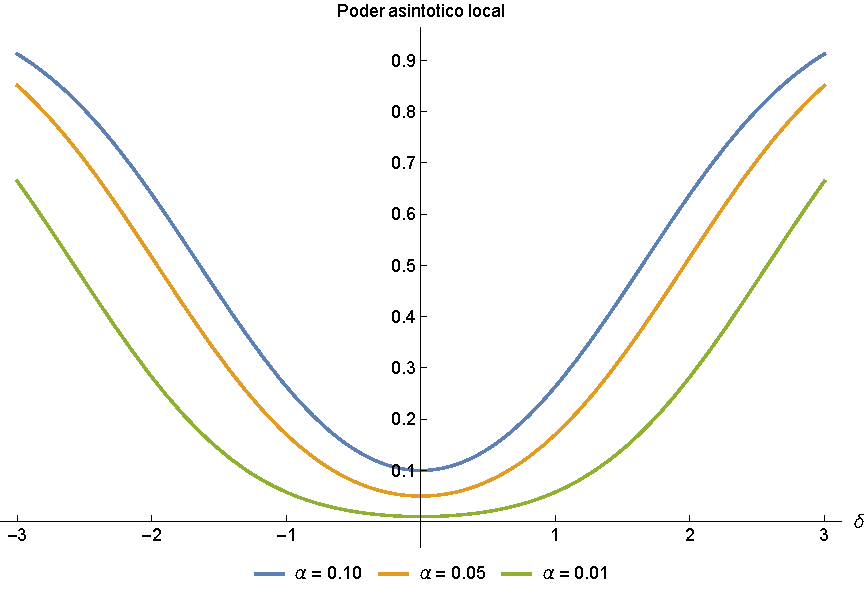
\includegraphics[width=0.65\textwidth]{figures/local_power_tstat.pdf}
     \caption{Poder asint\'otico local t-estad\'istico.}
     \end{figure}
\end{frame}
% --------------------------------------------------- Slide --
\begin{frame}
\frametitle{Hip\'otesis alternativa de una cola}
	\begin{small}
        \begin{itemize}
            \item \alert{Hip\'otesis nula}
            \begin{align*}
                H_0: \beta_j = \beta_{j,0}.
            \end{align*}
            \item  \alert{Hip\'otesis alternativa}
            \begin{align*}
                H_1: \beta_j > \beta_{j,0}.
            \end{align*}
            \item \alert{Test estad\'istico}: Estad\'istico t
            \begin{align*}
                t_N=\frac{\hat \beta_j-\beta_{j,0}}{s.e.(\hat \beta_j)} \dto_{H_0} Z \quad \text{donde}\quad Z \sim \N(0,1).
            \end{align*}
            \item  \alert{Valor cr\'itico} $c_\alpha=z_{1-\alpha}$:
            \begin{align*}
                \lim_{N\to \infty}\Pr(\text{Rechazar }H_0|H_0)=\lim_{N\to \infty} \Pr(t_N > c_\alpha|H_0)=\Pr(Z > c_\alpha)&=\alpha
                \iff c_\alpha=z_{1-\alpha}&.
            \end{align*}
            Si $\alpha=0.05$, entonces $c_\alpha=z_{0.95}=1.645$.
            \item \alert{Regla de decisi\'on}: Si $t_N>c_\alpha$, rechazamos $H_0$.
    	\end{itemize}
    \end{small}
\end{frame}
% --------------------------------------------------- Slide --
\begin{frame}
    \frametitle{Hip\'otesis alternativa de una cola}
	\begin{small}    
    \begin{itemize}
        \item \alert{Hip\'otesis nula}
        \begin{align*}
        H_0: \beta_j = \beta_{j,0}.
        \end{align*}
        \item  \alert{Hip\'otesis alternativa}
        \begin{align*}
        H_1: \beta_j < \beta_{j,0}.
        \end{align*}
        \item \alert{Test estad\'istico}: Estad\'istico t
        \begin{align*}
        t_N=\frac{\hat \beta_j-\beta_{j,0}}{s.e.(\hat \beta_j)} \dto_{H_0} Z \quad \text{donde}\quad Z \sim \N(0,1).
        \end{align*}
        \item  \alert{Valor cr\'itico} $c_\alpha=z_{1-\alpha}$:
        \begin{align*}
        \lim_{N\to \infty}& \Pr(\text{Rechazar }H_0|H_0) =\lim_{N\to \infty} \Pr(-t_N > c_\alpha|H_0)\\
        &=\lim_{N\to \infty}\Pr(t_N \leq -c_\alpha|H_0)=\alpha\\
        &\iff\Pr(Z \leq -c_\alpha)=\alpha \iff c_\alpha=z_{1-\alpha}.
        \end{align*}
    \end{itemize}
    \end{small}    
\end{frame}
% --------------------------------------------------- Slide --
\begin{frame}
    \frametitle{Hip\'otesis alternativa de una cola}
    \begin{itemize}
        \item \alert{Hip\'otesis nula}
        \begin{align*}
        H_0: \beta_j = \beta_{j,0}.
        \end{align*}
        \item  \alert{Hip\'otesis alternativa}
        \begin{align*}
        H_1: \beta_j < \beta_{j,0}.
        \end{align*}
        \item \alert{Test estad\'istico}: Estad\'istico t
        \begin{align*}
        t_N=\frac{\hat \beta_j-\beta_{j,0}}{s.e.(\hat \beta_j)} \dto_{H_0} Z \quad \text{donde}\quad Z \sim \N(0,1).
        \end{align*}
        \item  \alert{Valor cr\'itico} $c_\alpha=z_{1-\alpha}$.
        Si $\alpha=0.05$, entonces $c_\alpha=z_{0.95}=1.645$.
        \item \alert{Regla de decisi\'on}: Si $-t_N>c_\alpha$ \'o $t_N<-c_\alpha$, rechazamos $H_0$.
    \end{itemize}
\end{frame}
% --------------------------------------------------- Slide --
\begin{frame}
\frametitle{p-valor}
        \begin{itemize}
            \item Para $H_0: \beta_j = \beta_{j,0}$ y $H_1: \beta_j > \beta_{j,0}$, tenemos:
            \begin{align*}
                p_N=\Pr(T> T_N)=\Pr(Z>t_N)=1-\Phi(t_N).
            \end{align*}
            \item Para $H_0: \beta_j = \beta_{j,0}$ y $H_1: \beta_j < \beta_{j,0}$, tenemos:
            \begin{align*}
                p_N=\Pr(T> T_N)=\Pr(-Z>-t_N)=\Pr(Z< t_N)=\Phi(t_N)
            \end{align*}
        \end{itemize}
\end{frame}
%% --------------------------------------------------- Slide --
%\begin{frame}
%\frametitle{Ejemplo: Tama\~no de clase y rendimiento acad\'emico}
%        \begin{itemize}
%            \item Modelo
%            \begin{align*}
%                testscr_i = \beta_0 + \beta_1 \, str_i+\beta_2 el\_pct_i+u_i,
%            \end{align*}
%            \item \alert{Hip\'otesis nula}: El tama\~no de clase no tiene  efecto sobre el rendimiento acad\'emico.\\
%            Formalmente:
%            \begin{align*}
%                H_0: \beta_1=0.
%            \end{align*}
%            \item \alert{Hip\'otesis alternativa}: El tama\~no de clase tiene un efecto \alert{negativo} sobre el rendimiento acad\'emico.\\
%            Formalmente:
%            \begin{align*}
%                H_1: \beta_1 < 0.
%            \end{align*}
%        \end{itemize}
%\end{frame}
%% --------------------------------------------------- Slide --
%\begin{frame}[fragile]
%\frametitle{Tama\~no de clase y rendimiento acad\'emico}
%Salida de Stata\\
%\tiny{
%\begin{verbatim}
%    .     reg testscr str  el_pct, robust
%    
%    Linear regression                                      Number of obs =     420
%                                                           F(  2,   417) =  223.82
%                                                           Prob > F      =  0.0000
%                                                           R-squared     =  0.4264
%                                                           Root MSE      =  14.464
%    
%    ------------------------------------------------------------------------------
%                 |               Robust
%         testscr |      Coef.   Std. Err.      t    P>|t|     [95% Conf. Interval]
%    -------------+----------------------------------------------------------------
%             str |  -1.101296   .4328472    -2.54   0.011     -1.95213   -.2504616
%          el_pct |  -.6497768   .0310318   -20.94   0.000     -.710775   -.5887786
%           _cons |   686.0322   8.728224    78.60   0.000     668.8754     703.189
%    ------------------------------------------------------------------------------
%\end{verbatim}
%}
%\end{frame}
% --------------------------------------------------- Slide --
\section{Intervalo de confianza}

\begin{frame}
    \frametitle{Intervalo de confianza}
    \begin{itemize}
    	\item $\hat \beta_j$ es una estimaci\'on puntual de $\beta_j$.
    	\item Un concepto m\'as amplio, es un \alert{intervalo de confianza} $\hat C_{N}=[L_N,U_N]$ con el objetivo que $(1-\alpha)\%$ de la veces (\alert{nivel de cobertura o nivel de confianza}) dicho intervalo contenga a $\beta_j$:
$\lim_{N\to \infty}\Pr(\beta_j \in \hat C_N)=1-\alpha$
		\item Para un nivel de confianza de $1-\alpha$:
		$$\hat C_N=[\hat \beta_j-c_\alpha \,s.e.(\hat \beta_j),\hat \beta_j+c_\alpha \,s.e.(\hat \beta_j)]$$
    \end{itemize}
\end{frame}

%\begin{frame}
%	\frametitle{Intervalo de confianza}
%\end{frame}
%
%\begin{frame}
%	\frametitle{Intervalo de confianza}
%\end{frame}

\begin{frame}
    \frametitle{Intervalo de confianza}
    \begin{itemize}
        \item Para un nivel de confianza de $1-\alpha$:
        \begin{align*}
        \lim_{N\to \infty} \Pr\left(-c_\alpha<\frac{\hat \beta_j-\beta_j}{s.e.(\hat \beta_j)}< c_\alpha\right)&=\Pr\left(-c_\alpha<Z< c_\alpha\right)=1-\alpha
        \end{align*}
        donde $Z\sim \N(0,1)$ y $c_\alpha=z_{1-\alpha/2}$.
		Entonces,
        \begin{align*}
        &\lim_{N\to \infty} \Pr\left(-c_\alpha<\frac{\hat \beta_j-\beta_j}{s.e.(\hat \beta_j)}< c_\alpha\right)=\\
        &\lim_{N\to \infty}\Pr\left(\hat \beta_j-c_\alpha \, s.e.(\hat \beta_j)<\beta_j< \hat \beta_j+c_\alpha \,s.e.(\hat \beta_j)
        \right) =1-\alpha.
        \end{align*}
        Por lo tanto $\hat C_N=[\hat \beta_j-c_\alpha \,s.e.(\hat \beta_j),\hat \beta_j+c_\alpha \,s.e.(\hat \beta_j)]$
    \end{itemize}
\end{frame}


% --------------------------------------------------- Slide --
\begin{frame}[fragile]
	\frametitle{Estimaci\'on MCO: Tama\~no de clase y rendimiento acad\'emico}
	Salida de Stata
	\tiny{
		\begin{verbatim}
    .     reg testscr str  el_pct, robust
    
    Linear regression                                      Number of obs =     420
                                                           F(  2,   417) =  223.82
                                                           Prob > F      =  0.0000
                                                           R-squared     =  0.4264
                                                           Root MSE      =  14.464
    
    ------------------------------------------------------------------------------
                 |               Robust
         testscr |      Coef.   Std. Err.      t    P>|t|     [95% Conf. Interval]
    -------------+----------------------------------------------------------------
             str |  -1.101296   .4328472    -2.54   0.011     -1.95213   -.2504616
          el_pct |  -.6497768   .0310318   -20.94   0.000     -.710775   -.5887786
           _cons |   686.0322   8.728224    78.60   0.000     668.8754     703.189
    ------------------------------------------------------------------------------
\end{verbatim}
	}
	[-1.10 - 1.96 $\times$ .433, -1.10 + 1.96 $\times$ .433] = [-1.950, -.253] \\
	
\alert{Stata utilizar los valores cr\'iticos de la t-student}
\end{frame}
% --------------------------------------------------- Slide --
\section{Una restricci\'on lineal sobre m\'ultiples par\'ametros}
\begin{frame}
\frametitle{Una restricci\'on lineal sobre m\'ultiples par\'ametros}
        \begin{itemize}
            \item <1->\alert{Hip\'otesis nula}
            \begin{align*}
                H_0: r'\beta = \theta_0,
            \end{align*}
            donde $r$ es un vector de $K \times 1$ y $\theta_0$ es un escalar.
            \item \alert{Hip\'otesis alternativa}
            \begin{align*}
                H_1: r'\beta \neq \theta_0.
            \end{align*}
            \item <2-> \alert{Regla de decisi\'on}: Un estad\'istico $T_N$, un valor cr\'itico $c_\alpha$ y una regla de decisi\'on:
            \begin{enumerate}
                \item No rechazar $H_0$ si $T_N \leq c_\alpha$,
                \item Rechazar $H_0$ si $T_N > c_\alpha$.
            \end{enumerate}
        \end{itemize}
\end{frame}
% --------------------------------------------------- Slide --
\begin{frame}
\frametitle{Una restricci\'on lineal sobre m\'ultiples par\'ametros}
        \begin{itemize}
            \item  \alert{Test estad\'istico}: Estad\'istico t en valor absoluto
            \begin{align*}
                |t_N|=\left|\sqrt{N}\frac{r'\hat \beta-\theta_0}{\sqrt{r'\hat V r}} \right| \dto_{H_0} |Z| \quad \text{donde} \quad Z \sim \N(0,1).
            \end{align*}
        \end{itemize}
\end{frame}
%
%\begin{frame}
%\frametitle{Una restricci\'on lineal sobre m\'ultiples par\'ametros}
%\end{frame}

\begin{frame}
\frametitle{Una restricci\'on lineal sobre m\'ultiples par\'ametros}
        \begin{itemize}
            \item  \alert{Test estad\'istico}: Estad\'istico t en valor absoluto
            \begin{align*}
                |t_N|=\left|\sqrt{N}\frac{r'\hat \beta-\theta_0}{\sqrt{r'\hat V r}} \right| \dto_{H_0} |Z| \quad \text{donde} \quad Z \sim \N(0,1).
            \end{align*}
            \item [] \alert{Demostraci\'on}: Utilizando la distribuci\'on  asint\'otica normal:
            \begin{align*}
                \sqrt{N}(\hat \beta-\beta)&\dto \N(0,V).
            \end{align*}
            Utilizando el m\'etodo delta para $g(x)=r'x$,
            \begin{align*}
                \sqrt{N}(r'\hat \beta-r'\beta)&\dto \N(0,r'Vr),\\
                \implies \sqrt{N}(r'\hat \beta-\theta_0)&\dto_{H_0} \N(0,r'Vr).
            \end{align*}
            Utilizando el teorema de Slutsky,
            \begin{align*}
                t_N=\frac{\sqrt{N}(r'\hat \beta-\theta_0)}{\sqrt{r'\hat V r}}&\dto_{H_0} Z \sim \N(0,1).
            \end{align*}
        \end{itemize}
\end{frame}
% --------------------------------------------------- Slide --
\begin{frame}
\frametitle{Una restricci\'on lineal sobre m\'ultiples par\'ametros}
        \begin{itemize}
            \item  \alert{Test estad\'istico}: Estad\'istico t en valor absoluto
            \begin{align*}
            |t_N|=\left|\sqrt{N}\frac{r'\hat \beta-\theta_0}{\sqrt{r'\hat V r}} \right| \dto_{H_0} |Z| \quad \text{donde} \quad Z \sim \N(0,1).
            \end{align*}
            \item  \alert{Valor cr\'itico} $c_\alpha=z_{1-\alpha/2}$.
            \item \alert{Regla de decisi\'on}: Si $|t_N|>z_{1-\alpha/2}$, rechazamos $H_0$.
        \end{itemize}
\end{frame}
% --------------------------------------------------- Slide --
\begin{frame}
    \frametitle{Retornos de la educaci\'on (NLSY) (Blackburn and Neumark (QJE, 1992))}
    \begin{itemize}
        \item ?`Cu\'al es el efecto de un a\~no adicional de educaci\'on sobre los salarios?
        \item \alert{Datos}: Young Men's Cohort of the National Longitudinal Survey (NLSY). 5,225 individuos fueron encuestados por primera vez en 1966 a la edad de 14-24 a\~nos y luego en intervalos de uno o dos a\~nos. La muestra utilizada incluye solamente hombres que no son de raza negra, entrevistados en 1980 y que respondieron la pregunta sobre ingreso. Tama\~no de la muestra $N=935$.
    \end{itemize}
\end{frame}
        % Edad entre 28 y 38
        % En el a\~no 1968 les hicieron un IQ test y el KWW knowledge about the labor market
% --------------------------------------------------- Slide --
\begin{frame}
    \frametitle{Retornos de la educaci\'on (NLSY) (Blackburn and Neumark (QJE, 1992))}
    \begin{itemize}
        \item ?`Cu\'al es el efecto de un a\~no adicional de educaci\'on sobre los salarios?
        \item \alert{Variables}:
        \begin{itemize}
            \item Log del salario en 1980 (\emph{lwage}).
            \item A\~nos de educaci\'on (\emph{educ}).
            \item IQ test score realizado en  1968 (\emph{IQ}).
            \item A\~nos de experiencia laboral (\emph{exper}).
            \item A\~nos de tenure (trabajando en el mismo lugar) (\emph{tenure}).
            \item Dummies de est\'a casado (\emph{married}), vive en el sur de USA (\emph{south}) y vive en un \'area urbana (\emph{urban}).
        \end{itemize}
    \end{itemize}
\end{frame}
        % Edad entre 28 y 38
        % En el a\~no 1968 les hicieron un IQ test y el KWW knowledge about the labor market
        % --------------------------------------------------- Slide --
\begin{frame}
\frametitle{Modelo poblacional}
    \begin{itemize}
        \item  []
        \begin{small}
        \begin{align*}
            \log{wage_i} = \beta_0 + \beta_1 \, educ_i&+\beta_2 exper_i+\beta_3 tenure_i +\beta_4 IQ_i+x_i'\beta+u_i,
        \end{align*}
        \end{small}
        donde $x_i$ incluye regresores adicionales.
    \end{itemize}
\end{frame}
% --------------------------------------------------- Slide --
\begin{frame}[fragile]
\frametitle{Estimaci\'on MCO: Retornos de la educaci\'on (NLSY)}
Salida de Stata\\
\tiny{
\begin{verbatim}
    Linear regression                                      Number of obs =     935
                                                           F(  7,   927) =   52.82
                                                           Prob > F      =  0.0000
                                                           R-squared     =  0.2524
                                                           Root MSE      =  .36552
    
    ------------------------------------------------------------------------------
                 |               Robust
           lwage |      Coef.   Std. Err.      t    P>|t|     [95% Conf. Interval]
    -------------+----------------------------------------------------------------
            educ |   .0542004   .0072877     7.44   0.000     .0398982    .0685027
              IQ |   .0047061   .0009314     5.05   0.000     .0028783     .006534
           exper |   .0141831   .0032564     4.36   0.000     .0077923    .0205739
          tenure |   .0118061   .0025521     4.63   0.000     .0067976    .0168146
         married |   .2082196   .0395385     5.27   0.000     .1306243    .2858149
           south |  -.0974561   .0273761    -3.56   0.000    -.1511823   -.0437299
           urban |   .1714902   .0266955     6.42   0.000     .1190995    .2238809
           _cons |   5.047173   .1158771    43.56   0.000     4.819761    5.274585
    ------------------------------------------------------------------------------
\end{verbatim}
}
\end{frame}
% --------------------------------------------------- Slide --
\begin{frame}
\frametitle{Retornos de la educaci\'on (NLSY)}
        \begin{itemize}
            \item  Modelo poblacional
            \begin{small}
            \begin{align*}
                \log{wage_i} = \beta_0 + \beta_1 \, educ_i+\beta_2 exper_i+\beta_3 tenure_i+\beta_4 IQ_i+x_i'\beta+u_i,
            \end{align*}
            \end{small}
            \item \alert{Hip\'otesis nula}: Un a\~no adicional de experiencia y un a\~no adicional de tenure tienen el mismo efecto sobre el salario.\\
            Formalmente:
            \begin{align*}
                H_0: \beta_2=\beta_3 \text{ \'o } \beta_2 -\beta_3=0.
            \end{align*}
            \item \alert{Hip\'otesis alternativa}: Un a\~no adicional de experiencia y un a\~no adicional de tenure tienen efectos distintos sobre el salario.\\
            Formalmente:
            \begin{align*}
                H_1: \beta_2 \neq \beta_3  \text{ \'o } \beta_2 -\beta_3 \neq 0.
            \end{align*}
        \end{itemize}
\end{frame}

% --------------------------------------------------- Slide --
\begin{frame}[fragile]
\frametitle{Estimaci\'on MCO: Retornos de la educaci\'on (NLSY)}
Salida de Stata\\
\tiny{
\begin{verbatim}
.       matrix list e(V)

symmetric e(V)[8,8]
               educ          IQ       exper      tenure     married       south       urban       _cons
   educ   .00005311
     IQ  -3.605e-06   8.674e-07
  exper   .00001065  -3.073e-07    .0000106
 tenure  -1.898e-06   4.350e-08  -2.529e-06   6.513e-06
married   1.046e-06  -1.873e-06  -.00001243  -9.007e-06   .00156329
  south  -.00001055   5.755e-06   3.735e-06   7.042e-06   9.887e-06   .00074945
  urban  -.00003273   1.646e-06  -9.453e-06   5.571e-06   .00004269   .00011974   .00071265
  _cons  -.00043456   -.0000368  -.00020062  -2.857e-06  -.00103976  -.00084779  -.00023681    .0134275
\end{verbatim}
}
\end{frame}
% --------------------------------------------------- Slide --
%\begin{frame}
%\end{frame}
%
%\begin{frame}
%\end{frame}
%
%\begin{frame}
%\end{frame}

\begin{frame}
\frametitle{Retornos de la educaci\'on (NLSY)}
        \begin{itemize}
            \item Test estad\'istico
            \begin{align*}
                t_N&=\sqrt{N}\frac{\hat \beta_2-\hat \beta_3}{\sqrt{\hat V_{22}+\hat V_{33}-2 \hat V_{23}}},\\
                &=\frac{\hat \beta_2-\hat \beta_3}{\sqrt{\widehat{AVar}(\hat \beta_2)+\widehat{AVar}(\hat \beta_3)-2 \widehat{AVar}(\hat \beta_2,\hat \beta_3)}},\\
                &=\frac{.0142-.0118}{[.0000106 + 6.513\times 10^{-6}- 2(-2.529\times 10^{-6})]^\frac{1}{2}},\\
                &=0.505.
            \end{align*}
            \item $|t_N|<1.96$:  No rechazamos $H_0$.
            \item pvalor=$.614$
        \end{itemize}
\end{frame}

% --------------------------------------------------- Slide --
\begin{frame}[fragile]
    \frametitle{Estimaci\'on MCO: Retornos de la educaci\'on (NLSY)}
    Salida de Stata\\
    \small{
        \begin{verbatim}
.        test exper-tenure = 0

 ( 1)  exper - tenure = 0

       F(  1,   927) =    0.25
            Prob > F =    0.6138
        \end{verbatim}
    }
\end{frame}

%% --------------------------------------------------- Slide --
%\begin{frame}
%\frametitle{Modelo transformado}
%        \begin{itemize}
%            \item Definir $\theta=R'\beta - r$
%            \item \emph{Hip\'otesis nula}
%            \begin{align*}
%                H_0: \theta=0,
%            \end{align*}
%            \item [] \emph{Hip\'otesis alternativa}
%            \begin{align*}
%                H_1: \theta \neq 0.
%            \end{align*}
%            \item [] Transformar el modelo en funci\'on de $\theta$, y hacer un contraste sobre $\theta$.
%            \item [] <2->Demostraci\'on (sketch): Tarea 5.
%        \end{itemize}
%\end{frame}
%% --------------------------------------------------- Slide --
%\begin{frame}
%\frametitle{Retornos de la educaci\'on (NLSY)}
%        \begin{itemize}
%            \item Modelo poblacional
%            \begin{align*}
%                \log{wage_i} = \beta_0 + \beta_1 \, educ_i+\beta_2 exper_i+\beta_3 tenure_i+\beta_4 IQ_i+x_i'\beta+u_i,
%            \end{align*}
%            \item  Para el contraste $H_0: \beta_2 -\beta_3=0$, definimos
%            \begin{align*}
%                \theta=\beta_2 -\beta_3 \implies \beta_2=\theta+\beta_3.
%            \end{align*}
%            El modelo transformado es
%            \begin{align*}
%                \log{wage_i} =& \beta_0 + \beta_1 \, educ_i+\beta_3 (exper_i+tenure_i)+\theta\, exper_i\\
%                &+\beta_4 IQ_i+x_i'\beta+u_i.
%            \end{align*}
%            \item Contraste de hip\'otesis : $H_0: \theta=0$ vs. $H_1: \theta\neq 0$.
%        \end{itemize}
%\end{frame}
%% --------------------------------------------------- Slide --
%\begin{frame}[fragile]
%\frametitle{Estimaci\'on MCO: Retornos de la educaci\'on (NLSY)}
%Salida de Stata\\
%\tiny{
%\begin{verbatim}
%    Linear regression                                      Number of obs =     935
%                                                           F(  7,   927) =   52.82
%                                                           Prob > F      =  0.0000
%                                                           R-squared     =  0.2524
%                                                           Root MSE      =  .36552
%    
%    ------------------------------------------------------------------------------
%                 |               Robust
%           lwage |      Coef.   Std. Err.      t    P>|t|     [95% Conf. Interval]
%    -------------+----------------------------------------------------------------
%            educ |   .0542004   .0072877     7.44   0.000     .0398982    .0685027
%              IQ |   .0047061   .0009314     5.05   0.000     .0028783     .006534
%           exper |    .002377    .004709     0.50   0.614    -.0068646    .0116185
%    exper_tenure |   .0118061   .0025521     4.63   0.000     .0067976    .0168146
%         married |   .2082196   .0395385     5.27   0.000     .1306243    .2858149
%           south |  -.0974561   .0273761    -3.56   0.000    -.1511823   -.0437299
%           urban |   .1714902   .0266955     6.42   0.000     .1190995    .2238809
%           _cons |   5.047173   .1158771    43.56   0.000     4.819761    5.274585
%    ------------------------------------------------------------------------------
%   
%\end{verbatim}
%}
%\end{frame}
% --------------------------------------------------- Slide --
\section{M\'ultiples restricciones lineales}

%\begin{frame}
%\frametitle{M\'ultiples restricciones lineales}
%\end{frame}

\begin{frame}
\frametitle{M\'ultiples restricciones lineales}
        \begin{itemize}
            \item \alert{Hip\'otesis nula}
            \begin{align*}
                H_0: R'\beta = \theta_0,
            \end{align*}
            donde \alert{$R$ es una matriz de $K \times q$} con rango($R$) = $q$ y \alert{$\theta_0$ es un vector de $q \times 1$}.
            \item \alert{Hip\'otesis alternativa}
            \begin{align*}
                H_1: R'\beta \neq \theta_0.
            \end{align*}
            \item <2-> \alert{Regla de decisi\'on}: Un estad\'istico $T_N$, un valor cr\'itico $c_\alpha$ y una regla de decisi\'on:
            \begin{enumerate}
                \item No rechazar $H_0$ si $T_N \leq c_\alpha$,
                \item Rechazar $H_0$ si $T_N > c_\alpha$.
            \end{enumerate}
        \end{itemize}
\end{frame}
% --------------------------------------------------- Slide --
\begin{frame}
%\frametitle{M\'ultiples restricciones lineales}
        \begin{itemize}
            \item \alert{Test estad\'istico}: Estad\'istico de Wald
            \begin{align*}
                W_N=N(R'\hat \beta-\theta_0)'(R'\hat V R)^{-1}(R'\hat \beta-\theta_0) \dto_{H_0} \chi^2_q.
            \end{align*}
        \end{itemize}
\end{frame}
%La suma de q N(0,1)(independientes) al cuadrado es chi-cuadrado (q) 
        
%\begin{frame}
%%\frametitle{M\'ultiples restricciones lineales}
%\end{frame}
%
%\begin{frame}
%%\frametitle{M\'ultiples restricciones lineales}
%\end{frame}
%
%\begin{frame}
%%\frametitle{M\'ultiples restricciones lineales}
%\end{frame}

\begin{frame}
%	\frametitle{M\'ultiples restricciones lineales}
        \begin{itemize}
        	\item \alert{Demostraci\'on}: Utilizando la distribuci\'on  asint\'otica normal y el m\'etodo delta para $g(x)=R'x$:
        	\begin{align*}
        		\sqrt{N}(\hat \beta-\beta)&\dto \N(0,V),\\
        		\implies \sqrt{N}(R'\hat \beta-R'\beta)&\dto \N(0,R'VR),\\
        		\implies \sqrt{N}(R'\hat \beta-\theta_0)&\dto_{H_0} \N(0,R'VR).
        	\end{align*}
        	Utilizando el teorema de Slutsky,
        		\begin{align*}
        			(R'\hat V R)^{-1/2}\sqrt{N}(R'\hat \beta-R'\beta)&\dto \N(0,I_q).
        		\end{align*}
        	Utilizando el TFC y que $\sum_{k=1}^q z_k^2\sim \chi^2_q$ donde $z_k\sim\N(0,1)$ independientes,
        		\begin{align*}
        			W_N=N(R'\hat \beta-\theta_0)' (R'\hat V R)^{-1}(R'\hat \beta-\theta_0) \dto_{H_0} \chi^2_q.
        		\end{align*}
        \end{itemize}
    \end{frame}
    
% --------------------------------------------------- Slide --
\begin{frame}
%    \frametitle{M\'ultiples restricciones lineales}
    \begin{itemize}
        \item  \alert{Test estad\'istico}: Estad\'istico de Wald
        \begin{align*}
        W_N=N(R'\hat \beta-\theta_0)'(R'\hat V R)^{-1}(R'\hat \beta-\theta_0) \dto_{H_0} \chi^2_q.
        \end{align*}
        \item  \alert{Valor cr\'itico} $c_\alpha$:  $\Pr(\chi^2_q> c_\alpha)=\alpha$ \'o $\Pr(\chi^2_q\leq c_\alpha)=1-\alpha$.
        
        \item \alert{Regla de decisi\'on}: Si $W_N>c_\alpha$, rechazamos $H_0$.
        \item \alert{p-valor}: $\Pr(\chi^2_q>W_N)=1-G(W_N)$ donde $G(.)$ es la funci\'on de distribuci\'on de una $\chi^2_q$.
    \end{itemize}
\end{frame}
% --------------------------------------------------- Slide --
\begin{frame}
%\frametitle{M\'ultiples restricciones lineales}
        \begin{itemize}
            \item  \alert{Test estad\'istico}: Estad\'istico de Wald
            \begin{align*}
                W_N=N(R'\hat \beta-\theta_0)'(R'\hat V R)^{-1}(R'\hat \beta-\theta_0) \dto_{H_0} \chi^2_q.
            \end{align*}
            \item  El contraste con el test estad\'istico de Wald es \alert{consistente}.
            \item <2-> [] \alert{Demostraci\'on}
            \begin{align*}
                W_N&=N(R'\hat \beta-\theta_0)'(R'\hat V R)^{-1}(R'\hat \beta-\theta_0),\\
                &=N(R'\hat \beta-R'\beta)'(R'\hat V R)^{-1}(R'\hat \beta-R'\beta)\\
                &+N(R'\beta-\theta_0)'(R'\hat V R)^{-1}(R'\beta-\theta_0)+\\
                &+2N^{1/2}(R'\beta-\theta_0)'(R'\hat V R)^{-1/2} N^{1/2}(R'\hat V R)^{-1/2}(R'\hat \beta-R'\beta),\\
                &\dto_{H_1} \chi^2_q + \infty.
            \end{align*}
             El segundo t\'ermino domina ($N \times \text{ positivo}$) al tercer termino ($N^{1/2} \times \text{ positivo \'o negativo } \times N(0,I)$)
        \end{itemize}
        % .
\end{frame}
% --------------------------------------------------- Slide --
\begin{frame}
\frametitle{Retornos de la educaci\'on (NLSY)}
        \begin{itemize}
            \item  Modelo poblacional
            \begin{small}
            \begin{align*}
                \log{wage_i} = \beta_0 + \beta_1 \, educ_i+\beta_2 exper_i+\beta_3 tenure_i+\beta_4 IQ_i+x_i'\beta+u_i,
            \end{align*}
            \end{small}
            \item \alert{Hip\'otesis nula}: Ni la educaci\'on ni IQ tienen efecto sobre el salario.\\
            Formalmente:
            \begin{align*}
                H_0: \beta_1=0 \text{ y } \beta_4=0.
            \end{align*}
            \item  \alert{Hip\'otesis alternativa}: Educaci\'on \'o IQ tienen efecto sobre el salario (al menos uno de los dos).\\
            Formalmente:
            \begin{align*}
                H_1: \beta_1\neq 0 \text{ \'o } \beta_4\neq 0.
            \end{align*}
        \end{itemize}
\end{frame}
% --------------------------------------------------- Slide --
\begin{frame}[fragile]
\frametitle{Estimaci\'on MCO: Retornos de la educaci\'on (NLSY)}
Salida de Stata\\
\tiny{
\begin{verbatim}
    Linear regression                                      Number of obs =     935
                                                           F(  7,   927) =   52.82
                                                           Prob > F      =  0.0000
                                                           R-squared     =  0.2524
                                                           Root MSE      =  .36552
    
    ------------------------------------------------------------------------------
                 |               Robust
           lwage |      Coef.   Std. Err.      t    P>|t|     [95% Conf. Interval]
    -------------+----------------------------------------------------------------
            educ |   .0542004   .0072877     7.44   0.000     .0398982    .0685027
              IQ |   .0047061   .0009314     5.05   0.000     .0028783     .006534
           exper |   .0141831   .0032564     4.36   0.000     .0077923    .0205739
          tenure |   .0118061   .0025521     4.63   0.000     .0067976    .0168146
         married |   .2082196   .0395385     5.27   0.000     .1306243    .2858149
           south |  -.0974561   .0273761    -3.56   0.000    -.1511823   -.0437299
           urban |   .1714902   .0266955     6.42   0.000     .1190995    .2238809
           _cons |   5.047173   .1158771    43.56   0.000     4.819761    5.274585
    ------------------------------------------------------------------------------
\end{verbatim}
}
\end{frame}
% --------------------------------------------------- Slide --
\begin{frame}
    \frametitle{Estimaci\'on MCO: Retornos de la educaci\'on (NLSY)}
    \footnotesize
   \begin{align*}
   \frac{R'\hat V \,R} {N} &= 
   \left(
   \begin{array} {c c}
    \widehat \Avar(\hat\beta_{educ}) &  \widehat \Avar(\hat\beta_{educ}, \hat\beta_{IQ}) \\
    \widehat \Avar(\hat\beta_{educ}, \hat\beta_{IQ})  & \widehat \Avar(\hat\beta_{IQ})  
   \end{array}
   \right)  \\
   &=\left(
      \begin{array} {c c}
    .00005311&  -3.605\times 10^{-6} \\
    -3.605\times 10^{-6}  & 8.674\times 10^{-7} 
   \end{array}
   \right)\\
  \left[\frac{R'\hat V \,R} {N}\right]^{-1} &= \left(
      \begin{array} {c c}
    26228&  109005 \\
    109005 & 1605875
   \end{array}
   \right) \\
   W_N &= (.054 \, .0047)
  \left( \begin{array} {c c}
    26228&  109005 \\
    109005 & 1605875
   \end{array}\right)
   \left(\begin{array} {c }
    .054 \\
    .0047 
   \end{array}\right) = 168.22
    \end{align*}
\end{frame}
% --------------------------------------------------- Slide --
\begin{frame}[fragile]
\frametitle{Estimaci\'on MCO: Retornos de la educaci\'on (NLSY)}
Salida de Stata\\
\small{
\begin{verbatim}
        .      test educ IQ

 ( 1)  educ = 0
 ( 2)  IQ = 0

       F(  2,   927) =   84.11
            Prob > F =    0.0000
\end{verbatim}
}
\end{frame}
% --------------------------------------------------- Slide --
\begin{frame}
    \frametitle{Resultados reportados por Stata}
    \begin{itemize}
        \item  \alert{L\'imite de la distribuci\'on t y la distribuci\'on F}: Se puede demostrar que
        \begin{align*}
            t_{N-K} &\dto Z\sim \N(0,1),\\
           F_{q,N-K} &\dto \chi^2_q/q \implies q\, F_{q,N-K} \dto \chi^2_q  ,
        \end{align*}
        donde $t_{N-K}$ es una variable aleatoria con distribuci\'on t de Student con $N-K$ grados de libertad; $F_{q,N-K}$ es una variable aleatoria con distribuci\'on F de Fischer-Snedecor con $q$ grados de libertad en el numerador y $N-K$ grados de libertad en el denominador.
    \end{itemize}
\end{frame}
% --------------------------------------------------- Slide --
\begin{frame}
    \frametitle{Resultados reportados por Stata}
    \begin{itemize}
        \item Stata reporta en la salida de reg el \alert{p-valor de una t de Student para el estad\'istico t}; y reporta en la salida de test un \alert{estad\'istico $F_N=W_N/q$ con el p-valor de una F de Fischer-Snedecor}. Estos ajustes son irrelevantes en muestras grandes.
    \end{itemize}
\end{frame}


% --------------------------------------------------- Slide --
\begin{frame}
    \frametitle{Relaci\'on entre el estad\'istico F y el estad\'istico de Wald}
    \begin{itemize}
        \item  Estad\'istico F:
        \begin{align*}
        F_N=\frac{(SSR_N^r-SSR_N^u)/q}{SSR_N^u/N}
        \end{align*}
        donde $SSR_N^u$ es la suma de los residuos al cuadrado del modelo no restringido y $SSR_N^r$ es la suma de los residuos al cuadrado del modelo restringido.
        \item \alert{\'Unicamente bajo homoscedastidad} se cumple que 
        \begin{align*}
        F_N=W_N/q.
        \end{align*}
    \end{itemize}
\end{frame}

% --------------------------------------------------- Slide --
%\begin{frame}
%\frametitle{Relaci\'on entre el estad\'istico t y el estad\'istico de Wald}
%        \begin{itemize}
%            \item  Para una restricci\'on lineal: $W_N=t_N^2$.
%            \item  Si utilizamos dos estad\'isticos t con los valores cr\'iticos usuales obtenemos un nivel de significatividad err\'oneo.
%            \item  [] Ejemplo: $H_0: \beta_1 = 0$ y $\beta_2 = 0$ vs. $H_1: \beta_1 \neq 0$ \'o $\beta_2 \neq 0$.
%            \item  [] Rechazar si $|t_{1,N}|>1.96$ \'o  $|t_{2,N}|>1.96$ donde $t_{k,N}=\frac{\hat \beta_j}{s.e.(\hat \beta_j)}$.\\
%            Supongamos que $\Cov(\hat \beta_1,\hat \beta_2)=0$.
%             \begin{align*}
%                &\Pr_{H_0}(|t_{1,N}|>1.96 \text{ \'o } |t_{2,N}|>1.96)\\
%                &=1-\Pr_{H_0}(|t_{1,N}|\leq 1.96 \text{ y } |t_{2,N}|\leq 1.96),\\
%                &=1-\Pr_{H_0}(|t_{1,N}|>1.96) \times  \Pr_{H_0}(|t_{2,N}|>1.96)),\\                
%                 &= 1-(1-\alpha)^2=0.0975 \text{ \'o } \alert{9.75 \%}
%            \end{align*}
%            Si $\Cov(\hat \beta_1,\hat \beta_2)\neq 0$, el an\'alisis es m\'as complicado porque el tama\~no del test depende de la correlaci\'on.
%        \end{itemize}
%\end{frame}
% --------------------------------------------------- Slide --
\begin{frame}
\frametitle{Test de significatividad global}
        \begin{itemize}
            \item \alert{Hip\'otesis nula:} El modelo no tiene poder explicativo.
            \begin{align*}
                H_0: \beta_1 = ...=\beta_K = 0,
            \end{align*}
            \item [] \alert{Hip\'otesis alternativa}
            \begin{align*}
                H_1: \text{ Al menos un coeficiente es distinto de cero}.
            \end{align*}
            \item [] Test de Wald con $R=I_K$ y $\theta_0$ un vector de ceros de $K\times 1$.
            \item Es un test irrelevante con los tama\~nos de muestra actuales.
        \end{itemize}
\end{frame}
% --------------------------------------------------- Slide --
\begin{frame}[fragile]
\frametitle{Estimaci\'on MCO: Retornos de la educaci\'on (NLSY)}
Salida de Stata\\
\tiny{
\begin{verbatim}
    Linear regression                                      Number of obs =     935
                                                           F(  7,   927) =   52.82
                                                           Prob > F      =  0.0000
                                                           R-squared     =  0.2524
                                                           Root MSE      =  .36552
    
    ------------------------------------------------------------------------------
                 |               Robust
           lwage |      Coef.   Std. Err.      t    P>|t|     [95% Conf. Interval]
    -------------+----------------------------------------------------------------
            educ |   .0542004   .0072877     7.44   0.000     .0398982    .0685027
              IQ |   .0047061   .0009314     5.05   0.000     .0028783     .006534
           exper |   .0141831   .0032564     4.36   0.000     .0077923    .0205739
          tenure |   .0118061   .0025521     4.63   0.000     .0067976    .0168146
         married |   .2082196   .0395385     5.27   0.000     .1306243    .2858149
           south |  -.0974561   .0273761    -3.56   0.000    -.1511823   -.0437299
           urban |   .1714902   .0266955     6.42   0.000     .1190995    .2238809
           _cons |   5.047173   .1158771    43.56   0.000     4.819761    5.274585
    ------------------------------------------------------------------------------
\end{verbatim}
}
\end{frame}
% --------------------------------------------------- Slide --
\section{Restricciones no lineales}

%\begin{frame}
%\frametitle{Restricciones no lineales}
%\end{frame}


\begin{frame}
\frametitle{Restricciones no lineales}
        \begin{itemize}
            \item \alert{Hip\'otesis nula}
            \begin{align*}
                H_0: r(\beta) = \theta_0,
            \end{align*}
            donde $r$ es un vector de $q$ funciones reales $r_j:\SR^K\to\SR$ y $\theta_0$ es un vector de $q \times 1$.
            \item \alert{Hip\'otesis alternativa}
            \begin{align*}
                H_1: r(\beta) \neq \theta_0.
            \end{align*}
            \item <2-> \alert{Regla de decisi\'on}: Un estad\'istico $T_N$, un valor cr\'itico $c_\alpha$ y una regla de decisi\'on:
            \begin{enumerate}
                \item No rechazar $H_0$ si $T_N \leq c_\alpha$,
                \item Rechazar $H_0$ si $T_N > c_\alpha$.
            \end{enumerate}
        \end{itemize}
\end{frame}
% --------------------------------------------------- Slide --
\begin{frame}
\frametitle{Restricciones no lineales}
        \begin{itemize}
            \item  \alert{Test estad\'istico}: Estad\'istico de Wald
            \begin{align*}
                W_N=N\, (r(\hat \beta)-\theta_0)'(\hat R'\hat V \hat R)^{-1}(r(\hat \beta)-\theta_0) \dto_{H_0} \chi^2_q,
            \end{align*}
            donde $\hat R=\frac{\partial }{\partial \beta} r(\hat \beta)'$.
        \end{itemize}
\end{frame}
%
%\begin{frame}
%\frametitle{Restricciones no lineales}
%\end{frame}
%
%\begin{frame}
%\frametitle{Restricciones no lineales}
%\end{frame}
%
%\begin{frame}
%\frametitle{Restricciones no lineales}
%\end{frame}

% --------------------------------------------------- Slide --
\begin{frame}
\frametitle{Restricciones no lineales}
        \begin{itemize}
            \item  \alert{Test estad\'istico}: Estad\'istico de Wald
            \begin{align*}
                W_N=N\, (r(\hat \beta)-\theta_0)'(\hat R'\hat V \hat R)^{-1}(r(\hat \beta)-\theta_0) \dto_{H_0} \chi^2_q,
            \end{align*}
            donde $\hat R=\frac{\partial }{\partial \beta} r(\hat \beta)'$.
            \item [] \alert{Demostraci\'on}: Utilizando la distribuci\'on  asint\'otica normal y el m\'etodo delta para $r(x)$:
            \begin{align*}
                \sqrt{N}(\hat \beta-\beta)&\dto \N(0,V),\\
                \implies \sqrt{N}(r(\hat \beta)-r(\beta))&\dto \N(0,R'VR),\\
                \implies \sqrt{N}(r(\hat \beta)-\theta_0)&\dto_{H_0} \N(0,R'VR).
            \end{align*}
            Luego seguimos los mismos pasos que con restricciones lineales.
        \end{itemize}
\end{frame}
% --------------------------------------------------- Slide --
\begin{frame}
    \frametitle{Restricciones no lineales}
    \begin{itemize}
        \item  \alert{Test estad\'istico}: Estad\'istico de Wald
            \begin{align*}
            W_N=N\, (r(\hat \beta)-\theta_0)'(\hat R'\hat V \hat R)^{-1}(r(\hat \beta)-\theta_0) \dto_{H_0} \chi^2_q,
            \end{align*}
            donde $\hat R=\frac{\partial }{\partial \beta} r(\hat \beta)'$.
        \item  \alert{Valor cr\'itico} $c_\alpha$:  $\Pr(\chi^2_q> c_\alpha)=\alpha$ \'o $\Pr(\chi^2_q\leq c_\alpha)=1-\alpha$.
        \item \alert{Regla de decisi\'on}: Si $W_N>c_\alpha$, rechazamos $H_0$.
    \end{itemize}
\end{frame}

% --------------------------------------------------- Slide --
\begin{frame}
    \frametitle{Restricciones no lineales}
    \begin{itemize}
        \item El test t y el test de Wald funcionan bien para hip\'otesis lineales pero tienen problemas para hip\'otesis no lineales 
        \item [] Ambos tests no son invariantes a c\'omo formulamos $H_0$ \item [] Ejemplo: Podemos formular $H_0$ como $\beta_1=1$; $(\beta_1-1)^2=0$;$(\beta_1-1)^3=0$, y obtener conclusiones distintas.
    \end{itemize}
\end{frame}

% --------------------------------------------------- Slide --
\begin{frame}
	\frametitle{Efectos de la contaminaci\'on en los precios de las viviendas (Harrison and Rubinfeld (JEEM, 1978))}
	\begin{itemize}
		\item ?`Cu\'al es el efecto de una mayor concentraci\'on \'oxido nitroso en el aire en el precio de las viviendas?
            \item Modelo 
            \begin{small}            
            \begin{align*}
            \log(price)  = \beta_0 +\beta_{lnox} \,\log(nox) +\beta_{rooms}\, rooms + \beta_{stratio} \,stratio +u_i,
            \end{align*}
            \end{small}
            donde \emph{price} es el precio de la vivienda, \emph{nox} es la cantidad de \'oxido nitroso en el aire (contaminaci\'on), \emph{rooms} es el n\'umero de habitaciones y \emph{stratio} es el ratio estudiante/profesor en la comuna.
	\end{itemize}
\end{frame}
% --------------------------------------------------- Slide --
\begin{frame}[fragile]
	\frametitle{Estimaci\'on MCO: Efectos de la contaminaci\'on en los precios de las viviendas}
	Salida de Stata\\
	\tiny{
		\begin{verbatim}
.         reg lprice lnox rooms stratio, robust

Linear regression                                      Number of obs =     506
                                                       F(  3,   502) =  143.33
                                                       Prob > F      =  0.0000
                                                       R-squared     =  0.5760
                                                       Root MSE      =  .26729

------------------------------------------------------------------------------
             |               Robust
      lprice |      Coef.   Std. Err.      t    P>|t|     [95% Conf. Interval]
-------------+----------------------------------------------------------------
        lnox |  -.6453292   .0601569   -10.73   0.000    -.7635195   -.5271389
       rooms |    .256727   .0253943    10.11   0.000     .2068348    .3066192
     stratio |  -.0508733   .0047898   -10.62   0.000     -.060284   -.0414627
       _cons |   10.35946   .2627574    39.43   0.000     9.843218     10.8757
------------------------------------------------------------------------------
\end{verbatim}
	}
\end{frame}

    \begin{frame}
        \frametitle{Cambios grandes con logaritmo}
        \begin{itemize}
            \item Cuando los efectos marginales son grandes, $\frac{\partial \log{y}}{\partial x}$ puede que no sea una buena aproximaci\'on a $\frac{\frac{\Delta y}{y}}{\Delta x}$. Podemos calcular el cambio exacto.
        \end{itemize}
    \end{frame}
    
%    \begin{frame}
%        \frametitle{Cambios grandes con logaritmo}
%    \end{frame}

    \begin{frame}
        \frametitle{Cambios grandes con logaritmo}
        \begin{itemize}
            \item <1-> Cuando los efectos marginales son grandes, $\frac{\partial \log{y}}{\partial x}$ puede que no sea una buena aproximaci\'on a $\frac{\frac{\Delta y}{y}}{\Delta x}$. Podemos calcular el cambio exacto.
            \item <1-> Dado el modelo $\log y = \beta_0+\beta_1 x + u$, donde $u \independent x$. Podemos escribir
            \begin{align*}
            \E(y|x) = \exp(\beta_0+\beta_1 x) \E(\exp(u)),
            \end{align*}
            de donde
            \small
            \begin{align*}
            \frac{\E(y|x=\bar x+1)-\E(y|x=\bar x)}{\E(y|x=\bar x)}\times 100& = \left(\frac{\exp(\beta_0+\beta_1 (\bar x+1))}{\exp(\beta_0+\beta_1 (\bar x))}-1\right) \times 100\\
            &= (\exp(\beta_1)-1) \times 100.
            \end{align*}
        \end{itemize}
    \end{frame}

% --------------------------------------------------- Slide --
\begin{frame}
	\frametitle{Efectos de la contaminaci\'on en los precios de las viviendas (Harrison and Rubinfeld (JEEM, 1978))}
	\begin{itemize}
            \item  \alert{Hip\'otesis nula}
            \begin{align*}
                H_0: (\exp(\beta_{rooms})-1) \times 100 = 0.
            \end{align*}
            \item  \alert{Hip\'otesis alternativa}
            \begin{align*}
                H_1: (\exp(\beta_{rooms})-1) \times 100 \neq 0.
            \end{align*}
            \item  $r(\hat \beta)=(\exp(\hat\beta_{rooms})-1) \times 100=29.3$
            \item  $\hat R=\exp(\hat\beta_{rooms}) \times 100$
            \item $\frac{1}{N} \hat R'\hat V \hat R= \exp(\hat\beta_{rooms}) 100\times  \widehat{AVar}(\hat\beta_{rooms}) \times  \exp(\hat\beta_{rooms}) 100 = 10.8$
            \item $W_N=N\frac{r(\hat \beta)^2}{\hat R'\hat V \hat R} = \frac{29.3^2}{10.8} = 79.5$                      
	\end{itemize}
\end{frame}
% --------------------------------------------------- Slide --
\begin{frame}[fragile]
	\frametitle{Estimaci\'on MCO: Efectos de la contaminaci\'on en los precios de las viviendas}
	Salida de Stata\\
	\tiny{
		\begin{verbatim}
.         nlcom (exp(_b[rooms]) -1)*100

_nl_1:  (exp(_b[rooms]) -1)*100

------------------------------------------------------------------------------
      lprice |      Coef.   Std. Err.      t    P>|t|     [95% Conf. Interval]
-------------+----------------------------------------------------------------
       _nl_1 |   29.26922   3.282702     8.92   0.000     22.81969    35.71875
------------------------------------------------------------------------------

.         testnl  (exp(_b[rooms]) -1)*100 = 0

(1)  (exp(_b[rooms]) -1)*100 = 0

F(1, 502) =       79.50
 Prob > F =        0.0000
\end{verbatim}
	}
\end{frame}

\end{document}